\section{Theorie}
\label{sec:Theorie}
Ziel des Versuchs ist es die Quantennatur der Elektronenhülle eines Atoms nachzuweisen.
Mittels Elektronenstoßexperimenten ist es Beispielsweise möglich diese aufzuzeigen.
Stößt ein Elektron mit der bestimmten Anregungsnergie auf ein Atom, so wird das Atom aus dem Grundzustand auf seinen ersten angeregten Zustand gehoben.
Die Stoßpartner stoßen bei diesem Vorgang inelastisch.
Besitzt das Elektron nicht dem geeigneten Energiewert, dann stoßen Elektron und Atom elastisch und das Atom wird nicht angeregt.

\subsection{Der Frank-Hertz-Versuch}
Der Franck-Hertz-Versuch besteht aus einem evakuiertem Gefäß in dem sich Quecksilberdampf befindet.
Die Dampfdichte kann über die Umgebungstemperatur reguliert werden.
In das Gefäß ist ein Draht aus einem hochschmelzenden Metall eingeführt.
Wird dieser auf Rotglut erhitzt, so treten Elektronen aus, welchen den Draht wie eine Wolke umgeben.
Eine netzförmige Elektrode ist dem Draht gegenüber angebracht, an welcher eine positive Gleichspannung $U_B$ angelegt ist.
Durchlaufen die Elektronen die Strecke zwischen Glühdraht und Elektrode, so erhalten sie die kinetische Energie
\begin{equation}
  \label{eq:ekin}
  E_{kin} = e_0 U_B  ,
\end{equation}
wenn ihre Geschwindigkeit zu Beginn $v= 0$ beträgt.
Hinter der Beschleunigerelektrode befindet sich eine Auffängerelektrode.
Die Auffängerelektrode besitzt eine geringe Spannung gegenüber der der Beschleunigungsspannung.
Deshalb können nur Elektronen gegen das so entstehende Bremsfeld anlaufen, deren Geschwindigkeitskomponente in $z$-Richtung die Ungleichung
\begin{equation}
  \label{eq:ungl}
  \frac{m_0}{2}v_z^2 \geq e_0 U_A
\end{equation}
erfüllt.
Der Auffängerstrom $I_A$ kann mit einem geeignetem Messinstrument gemessen werden.
Im Beschleungigungraum befinden sich Hg-Atome.
Zwischen diesen und den Elektronen kommt es zu Zusammenstößen.
Ist die Energie der stoßenden Elektronen relativ gering, so treten elastische Stöße auf.
Aufgrund des großen Massenunterschieds der Stoßpartner ist die Energieübertragung des Elektrons an das Hg-Atom vernachlässigbar gering.
Im zentralen Stoß beträgt die übertragene Energie
\begin{equation}
  \label{eq:betrag}
  \symup\Delta E = \frac{4 m_0 M}{(m_0 + M)^2} E \approx \num{1.1e-5} E  .
\end{equation}
Die Richtungsänderungen, welche das Elektron erfährt können gravierend sein.
Erreicht die Elektronenenergie durch erhöhen von $U_B$ einen Wert der größer oder gleich der Energiedifferenz, zwischen dem ersten angeregten und dem Grundzustand des Hg-Atoms ist, so kann das Elektron das Hg-Atom anregen.
Das Elektron überträgt dabei genau den Energiebetrag $E_1 - E_0$ auf die Elektronenhülle des Hg-Atoms und behält den Restbetrag.
Das Hg-Atom befindet sich dann in dem ersten angeregtem Zustand.
Es geht mit einer Relaxationszeit in der Größenordnung $\SI{e-8}{\second}$ in den Grundzustand zurück, dabei emittiert es ein Photon mit der Energie
\begin{equation}
  \label{eq:phot}
  h\nu = E_1 -E_0    .
\end{equation}
Die Anregung des Hg-Atoms kann beobachtet werden indem der Auffängerstrom $I_A$ in Abhängigkeit der Beschleunigungsspannung $U_B$ gemessen wird.
Wird die Beschleunigungsspannung, ausgehend von Null, erhöht, dann Bewegen sich die von dem Glühdraht emittierten Elektronen weg von diesem.
Da eine anwachsende Zahl an Elektronen die Auffängerelektrode erreicht steigt der Auffängerstrom $I_A$ an.
Erreicht oder überschreitet die Energie der Elektronen den Wert $E_1-E_0$ ein wenig, sinkt der Auffängerstrom rapide ab.
Die Elektronen führen unelastische Stöße mit den Hg-Atomen durch, bei welchen sie fast ihre gesamte Energie übertragen.
Die Elektronen sind nicht mehr in der Lage gegen das Bremsfeld anzulaufen.
Wird die Energie weiter über die Beschleunigungsspannung gesteigert, so ist es ihnen wieder möglich Stöße mit den Hg-Atomen auszuführen.
Der Auffängerstrom steigt wieder an bis die Elektron erneut den Betrag $E_1-E_0$ erreicht haben.
Der Theoretische Verlauf des Auffängerstroms gegen die Beschleunigungsspannung ist in Abbildung \ref{fig:besch} dargestellt.
\begin{figure}[H]
  \centering
  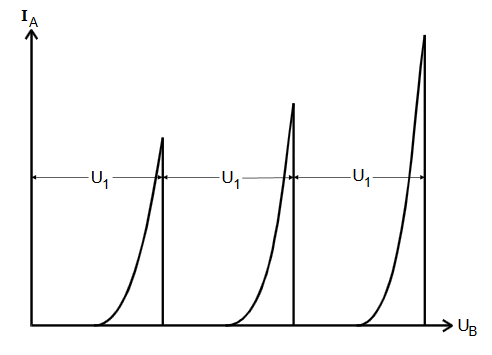
\includegraphics[width=0.8\textwidth]{content/theoriekurve.png}
  \caption{Idealisierter Zusammenhang zwischen Auffängerstrom und Beschleunigungsspannung\cite{v601}.}
  \label{fig:besch}
\end{figure}

\noindent Der Abstand zweier Maxima ist gleich dem ersten Anregungspotentials des Hg-Atoms:
\begin{equation}
  \label{eq:pot}
  U_1 = \frac{E_1 - E_0}{e_0}  .
\end{equation}
 \subsection{Einflüsse auf die Gestalt der Kurve}
Die tatsächlich gemessene Kurve weicht von der idealisierten Darstellung in Abbildung \ref{fig:besch} ab.
Dies geschieht aufgrund von verschiedenen Einflüssen.
\subsubsection{Einfluss des Kontaktpotentials}
In Glühdraht und Beschleunigerelektrode werden Materialien mit unterschiedlichen Austrittsarbeiten verwendet.
Damit eine hohe Elektronenemissionsrate erreicht wird, wird für den Glühdraht ein Material mit kleinerer Austrittsarbeit $\phi_G$ als die Austrittsarbeit $\phi_B$ der Beschleunigerelektrode verwendet.
Das tatsächliche Beschleunigunspotential ist dann häufig von der angelegten Spannung verschieden und kann mit folgender Gleichung beschrieben werden:
\begin{equation}
  U_\text{B,eff}= U_B-\frac{1}{e_0}(\phi_B -\phi_G) .
\end{equation}
Die Frank-Hertz-Kurve ist um den Wert
\begin{equation}
  \label{eq:k}
  K = U_B - U_\text{eff} = \frac{\phi_B - \phi_G}{e_0}
\end{equation}
verschoben, wobei $U_\text{eff}$ das effektive Potential darstellt.
Dieser wird als Kontaktpotential bezeichnet.
\subsubsection{Einfluss des Energie-Spektrums der Elektronen}
Die Leitungselektronen in einem Metall besitzen bereits ein Energiespektrum, welches als Fermi-Dirac-Verteilung bezeichnet wird.
Die Elektronen treten daher bei Glühemission mit unterschiedlichen Geschwindigkeiten aus dem Glühdraht aus.
Es gibt keinen disktreten Energiewert für alle Elektronen, sondern eine statistische Energieverteilung.
Es gibt keine Unstetigkeiten in der Kurve.
Die Kurve fällt nicht wie in Abbildung \ref{fig:besch} nach einem Maximum mit negativ unendlicher Steigung auf Null, sondern nähert sich stetig einem Stromminimum.
\subsubsection{Einfluss des Dampfdrucks}
Notwendig für die Beobachtung der Franck-Hertz-Kurve ist ein bestimmter Stoßwahrscheinlichkeitsbereich zwischen Elektronen und Hg-Atomen.
Damit dies realisiert werden kann muss die mittlere freie Weglänge $\bar{w}$ klein gegen den Abstand zwischen Kathode und Beschleunigungselektrode sein.
Die Größe $\bar{w}$ kann über den Sättigungsdampfdruck $p_{sät}$ reguliert werden.
Es gilt:
\begin{equation}
  \label{eq:laeng}
  \bar{w}[\si{\centi\meter}] =\frac{\num{0.0029}}{p_{sät}}[\text{p in } \si{\milli\bar}]
\end{equation}
Der Sättigungsdampfdruck kann über die Innentemperatur geregelt werden.
Dieser kann über
\begin{equation}
  \label{eq:druck}
  p_{sät}(T) = \num{5.5e7} \exp\left(\frac{\num{-6876}}{T}\right)
\end{equation}
berechnet werden.
Wird der optimale Bereich stark unterschritten, dann wächst die Wahrscheinlichkeit, dass die Elektronen ohne Wechselwirkung von der Katode bis zu der Auffängerelektrode durchlaufen.
Wird der optimale Bereich stark überschritten, dann steigt zwar die Wahrscheinlichkeit, dass die Elektronen mit den Hg-Atomen wechselwirken,
es kommt aber auch zu elastischen Stößen, welche die Richtung der Elektronen ändern.
Die Zahl der Elektronen, welche die Auffängerelektrode erreichen, nimmt ab.
